\chapter{Proceso de Potabilización}
\label{ch:ProcesoOoapas}

El presente trabajo de tesis fue posible gracias al apoyo del OOAPAS (Organismo Operador de Agua Potable, Alcantarillado y Saneamiento de Morelia). Dicho organismo del gobierno municipal de la ciudad de Morelia nos permitió 
durante el año 2024 el acceso a una de sus plantas de potabilización, en la cual se nos permitió trabajar en su laboratorio de muestreo para realizar la recolección de los datos sobre las muestras obtenidas de las diferentes
etapas del proceso consideradas significativas para los propósitos establecidos en los objetivos y la metodología. En este capítulo se dará una descripción de las etapas que componen el proceso de potabilización llevado a 
cabo en esta planta, las cuales abarcan desde el agua que se recibe desde la presa captadora de agua que abastece a estas instalaciones hasta el producto final generado por el proceso, dicho producto es agua potable apta 
para su distribución.

En la \autoref{fig:figura947_1} se muestra un diagrama de las etapas que componen el proceso de potabilización estudiado.

La \autoref{fig:figura947_1} presenta el flujo del proceso de potabilización a través de sus diferentes etapas, además de indicar con una etiqueta en color rojo las fases del proceso que han sido previamente elegidas para 
la recolección de muestras.

\clearpage

\begin{figure}[h]
	\centering
	\includegraphics[scale=1]{imgss216.png}
	\caption{Etapas del proceso de potabilización}
	\label{fig:figura947_1}
\end{figure}

En la \autoref{fig:figura900_1}, se muestra el pozo que se tiene en la planta potabilizadora que permite acceder y poder extraer muestras del agua cruda que proviene 
directamente de la presa de Cointzio. La utilidad de poder extraer muestras de agua cruda radica en poder analizar sus parámetros fisicoquímicos y biológicos, y así 
poder conocer cuáles son las condiciones que se tienen en un momento específico en la presa en la cual se recolecta el agua, lo que permite determinar el nivel de 
contaminación presente en dicha presa. Sin embargo, el hecho de que pudiera llegar a la planta potabilizadora agua con niveles altos de contaminación, 
no necesariamenete indicaría que en la presa existiese por ejemplo un problema de que dicho cuerpo de agua tuviera en sí mismo problemas de contaminación. Podría ser 
incluso que los canales que transportan el agua de la presa a la planta requieran algún procedimiento de limpieza o retiro de basura que pudiera tener acumulada por el paso del tiempo.

Por ejemplo, durante los muestreos realizados en el mes de agosto de 2024, el agua recolectada de este pozo presentaba un nivel de contaminación muy alto debido a que, al ser época de lluvias, muchos contaminantes tanto 
artificiales como naturales son arrastrados por el agua de lluvia y logran filtrarse al agua que viaja desde la Presa de Cointzio hasta la planta de potabilización. Este sería un ejemplo de cómo factores externos pueden 
modificar de manera drástica la calidad del agua que se recibe en la planta, y por lo cual resulta imprescindible monitorear los diferentes parámetros en esta etapa del proceso para poder identificar si algún cambio es necesario 
en el proceso de potabilización para compensar los efectos sobre la calidad del agua cruda provocados por factores diversos.  

\clearpage

\begin{figure}[h]
	\centering
	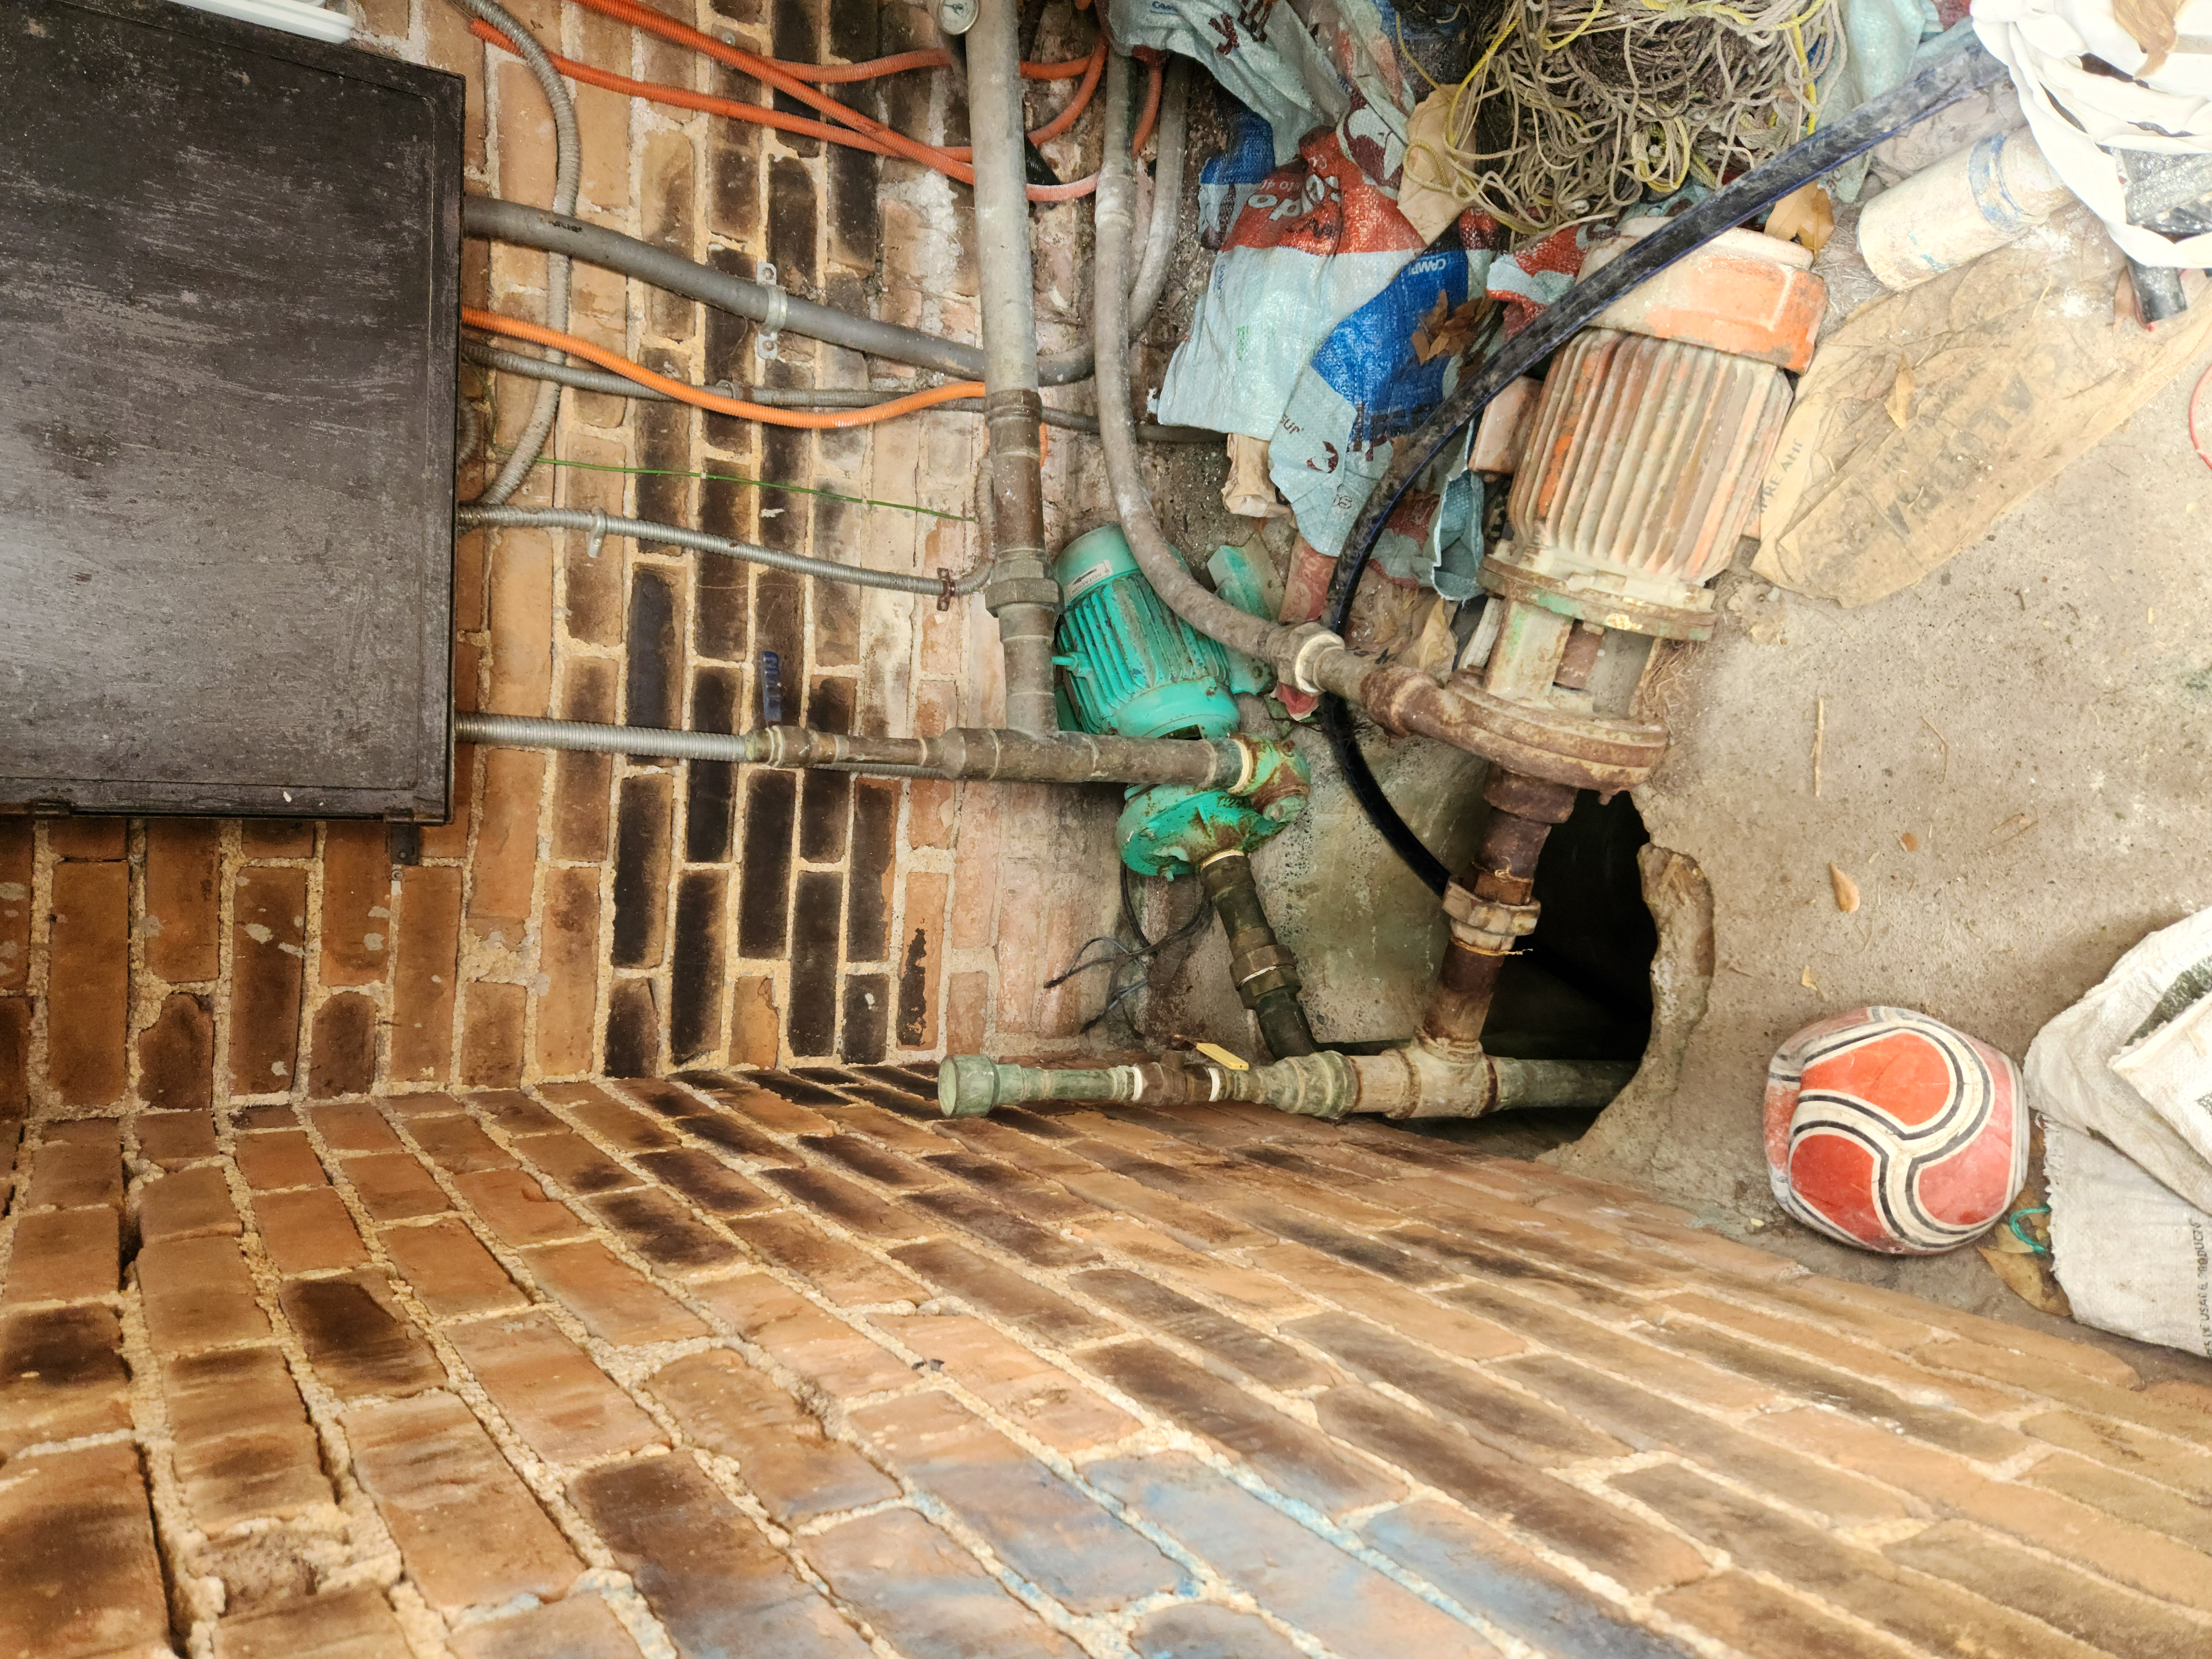
\includegraphics[scale=0.05,angle=-90]{imgss12.jpg}
	\caption{Pozo de entrada de agua proveniente de la Presa de Cointzio}
	\label{fig:figura900_1}
\end{figure}

Una vez que el agua cruda ha ingresado a la planta, de las primeras acciones que se realizan es iniciar a inyectar agentes químicos desinfectantes, así como otras sustancias que ayudan a procesar los contaminantes presentes y 
posteriormente poder eliminarlos. Por otra parte, la razón de adicionar al agua sustancias desinfectantes desde el inicio del proceso es que se busca que dichas sustancias actuén durante todo el proceso y tengan una ventana de 
tiempo más amplia para poder cumplir su función.

En la \autoref{fig:figura900_2} se muestra el área donde se introduce al proceso el compuesto coagulante Sulfato de Aluminio. 

\begin{figure}[h]
	\centering
	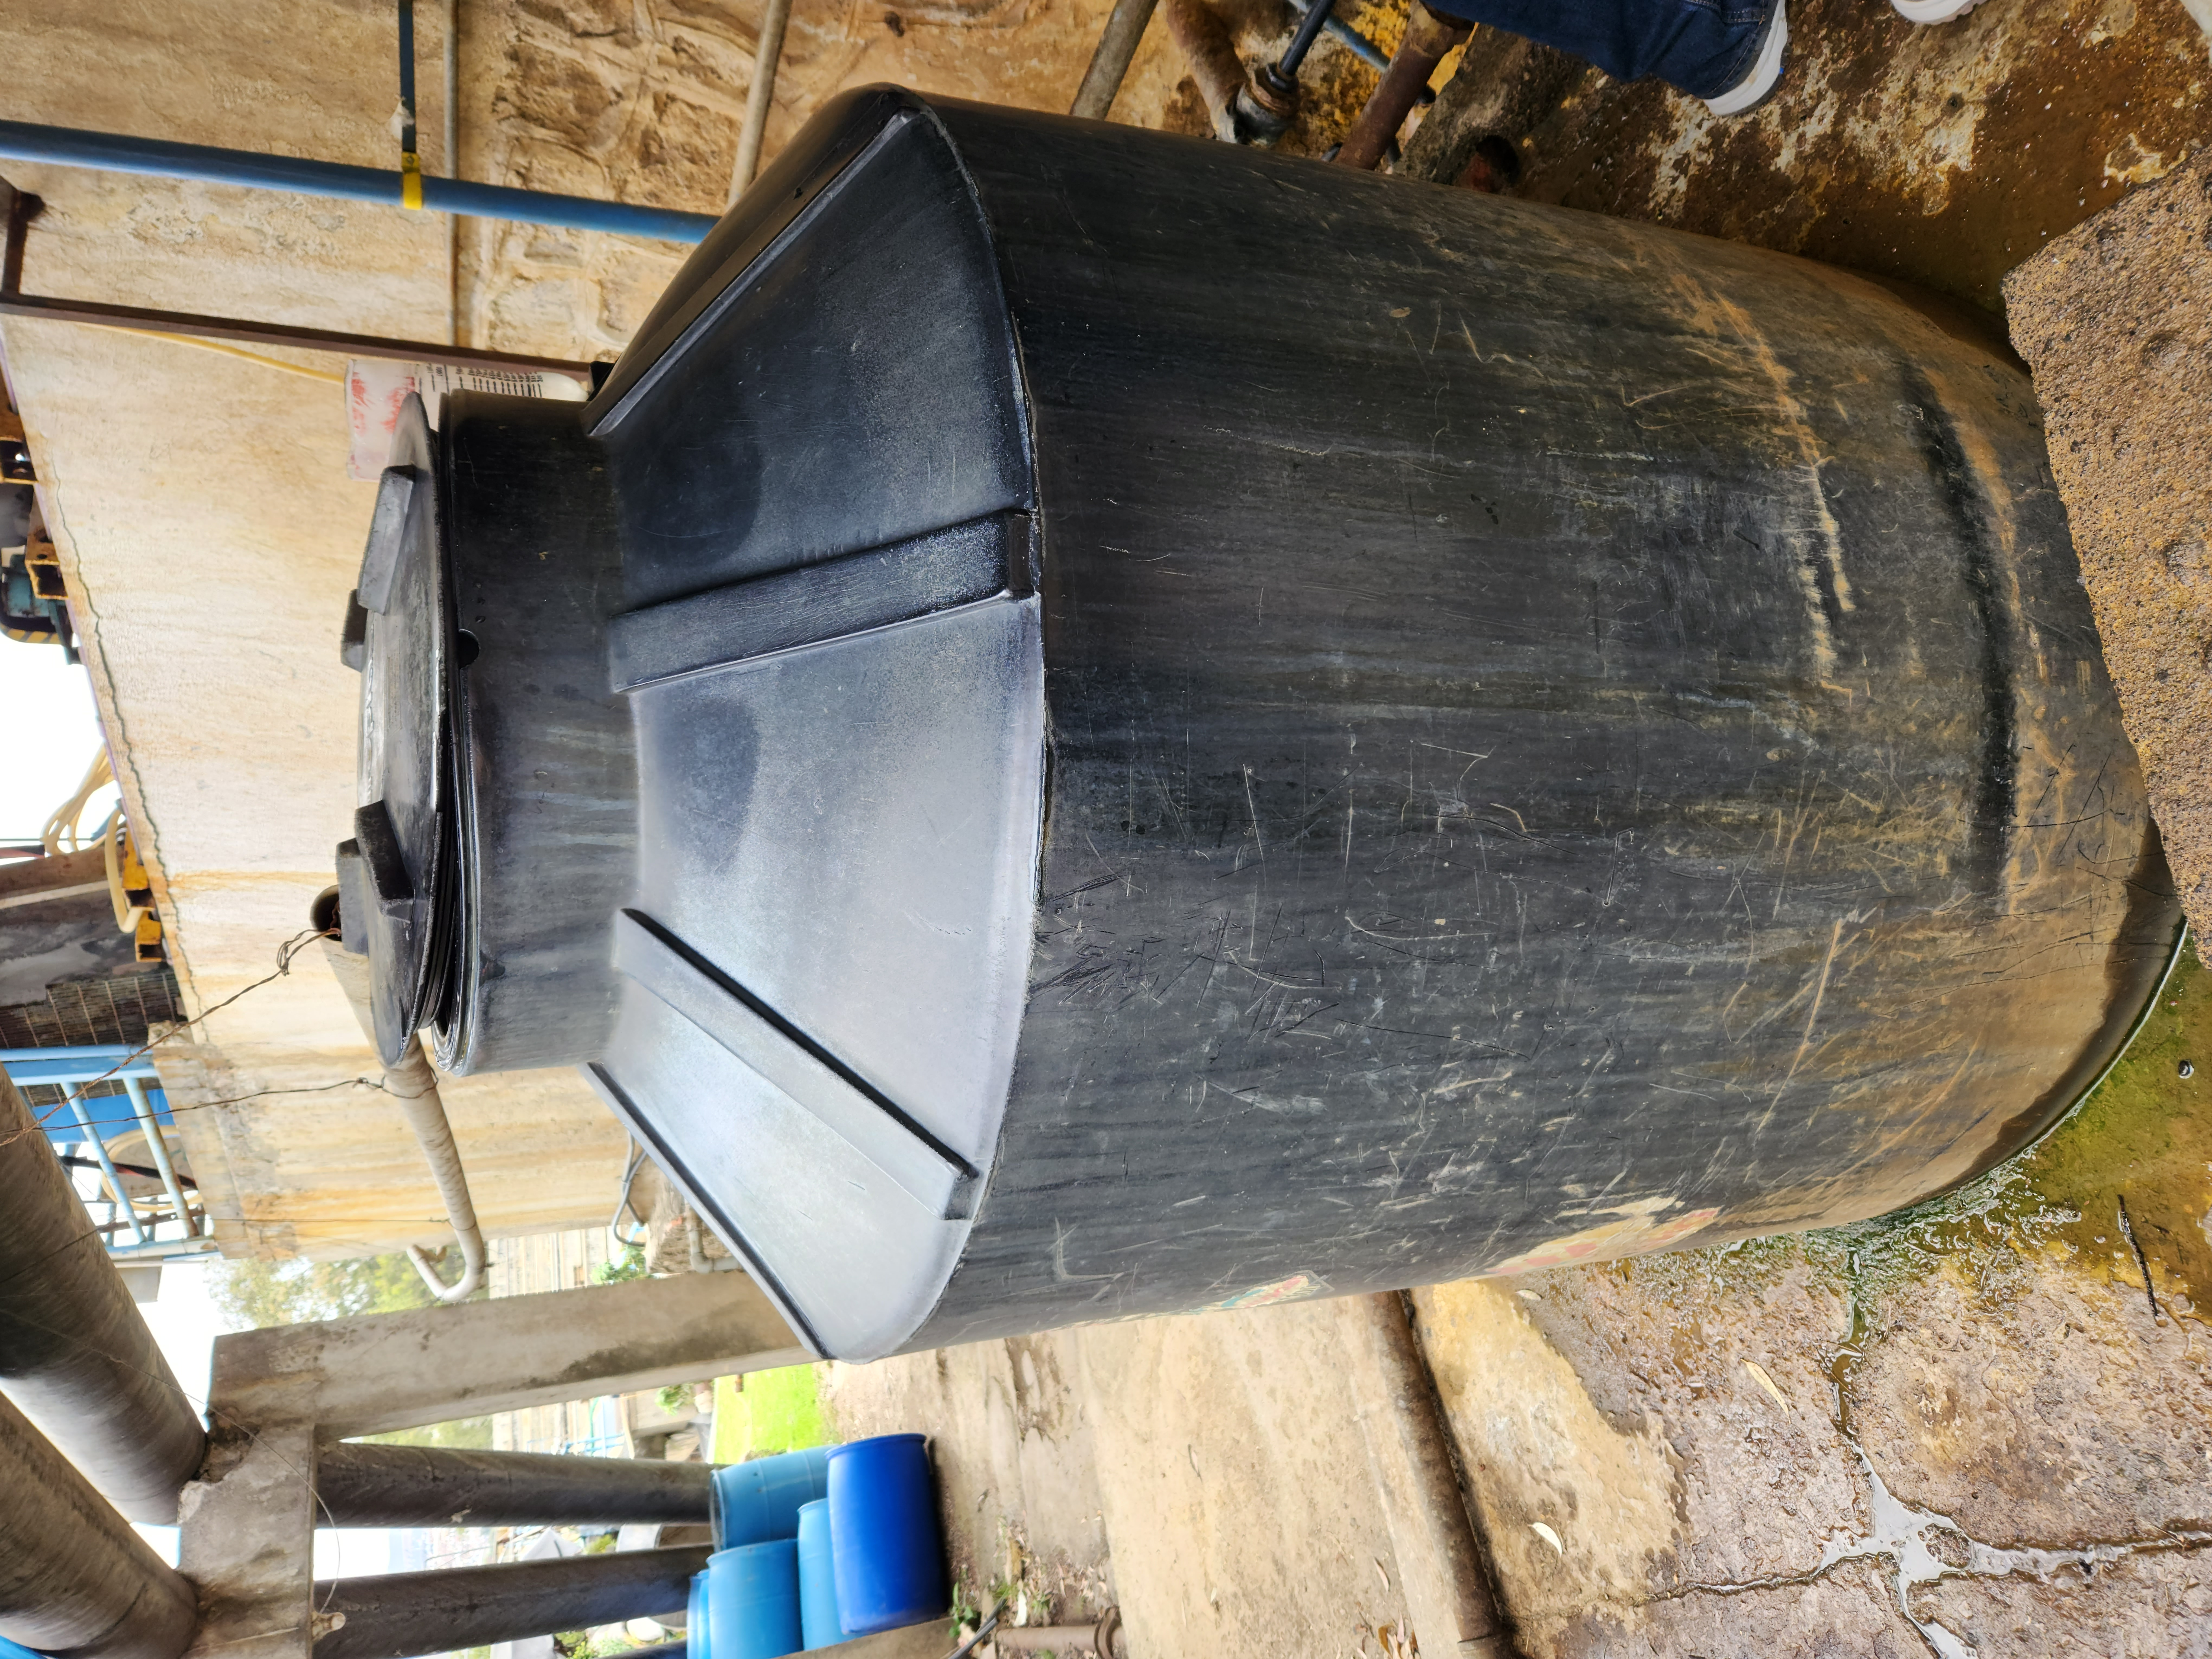
\includegraphics[scale=0.05,angle=-90]{imgss13.jpg}
	\caption{Adición del coagulante Sulfato de Aluminio}
	\label{fig:figura900_2}
\end{figure}

\clearpage

Un proceso de coagulación permite la neutralización de los sólidos suspendidos en al agua que se encuentren cargados eléctricamente. Es decir, el reactivo coagulante 
agregado al agua presenta una carga eléctrica neta positiva, lo cual permite neutralizar la carga neta en el líquido al eliminar dicha carga negativa que viene en 
los sólidos suspendidos en el agua.

El hecho de poder eliminar la carga eléctrica neta presente permite que las partículas con el mismo tipo de carga no sufran constantemente fuerzas de repulsión entre ellas, logrando así posteriormente tener la posibilidad 
de agrupar todos estos residuos, lo cual facilita su separación al ya no tener dispersos a la mayor cantidad de dichos contaminantes.

En la \autoref{fig:figura900_3} se muestra la adición del compuesto floculante catiónico.

\begin{figure}[h]
	\centering
	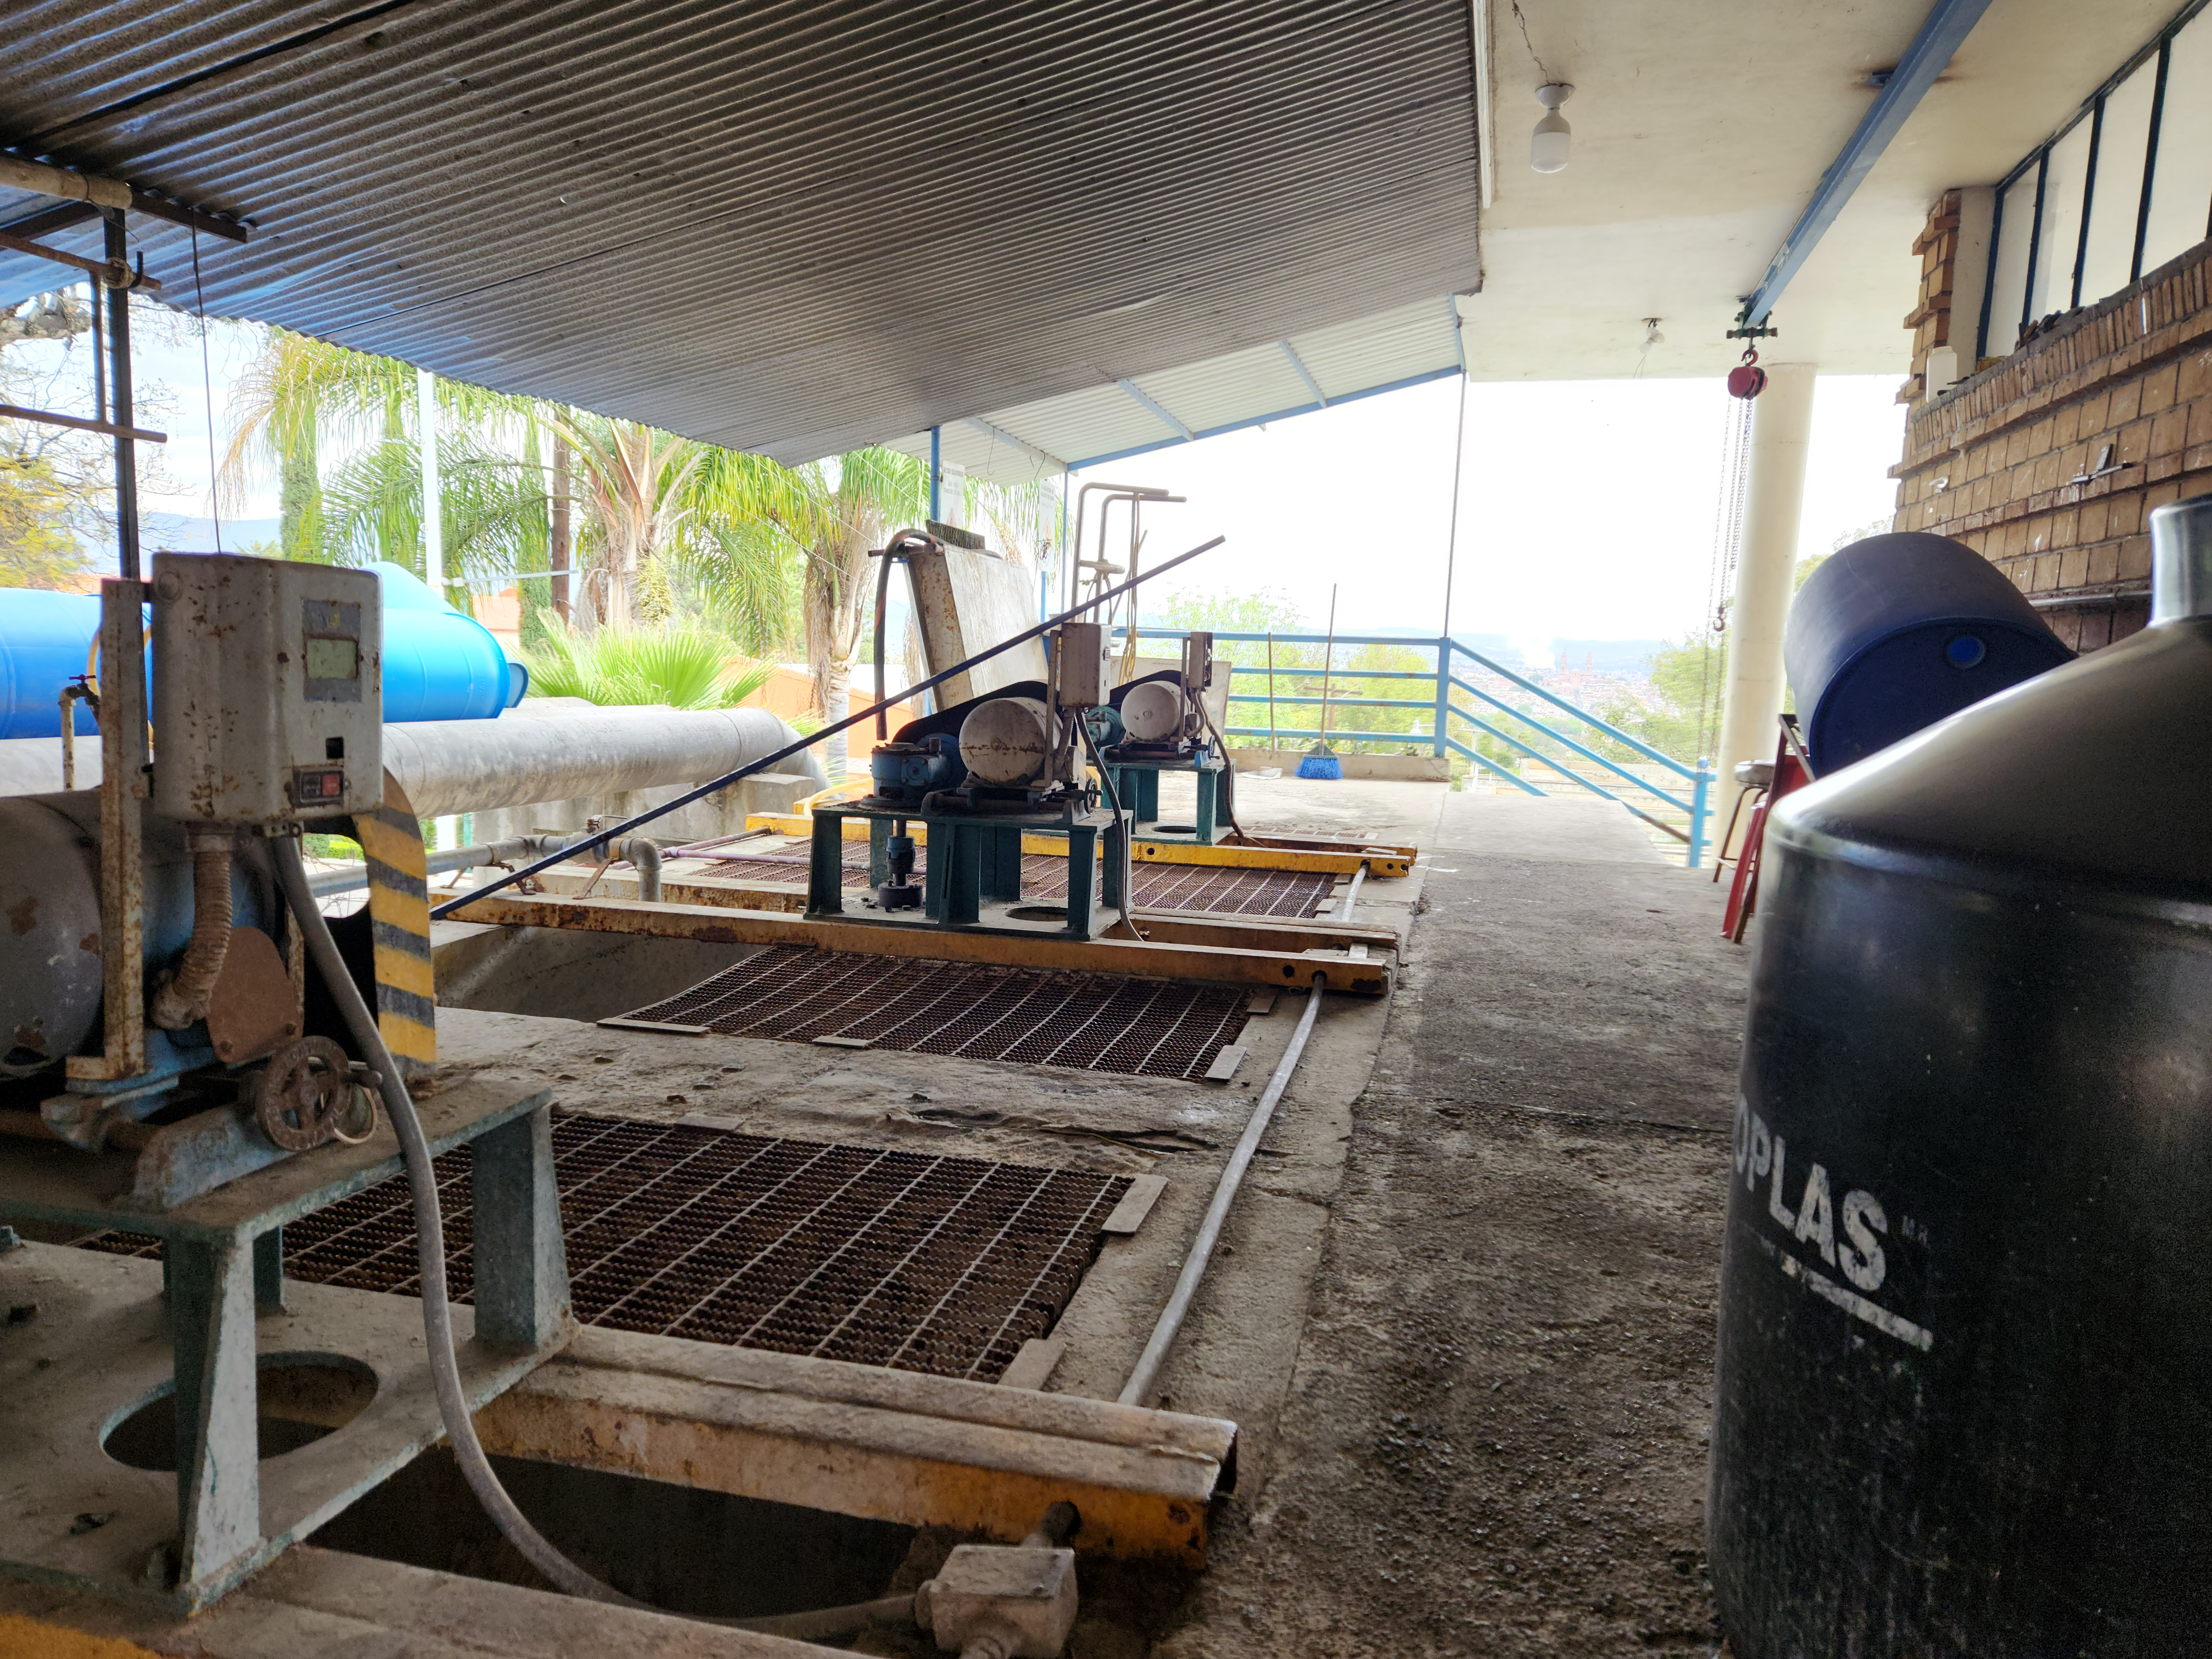
\includegraphics[scale=0.05,angle=0]{imgss14.jpg}
	\caption{Adición del floculante catiónico}
	\label{fig:figura900_3}
\end{figure}

La función que realiza este reactivo es la de aglomerar partículas pequeñas o coloidales que se encuentran presentes en el agua, con el objetivo de lograr la formación 
de flóculos más grandes y densos, lo que posteriormente facilita su separación del agua en etapas posteriores del proceso.

Dado que en el agua cruda proveniente de la presa se tienen presentes una diversa cantidad de tipos de contaminantes, particularmente en el factor de sus dimensiones físicas, al tener partículas contaminantes de tamaño pequeño 
resulta conveniente poder agruparlas o juntarlas para facilitar su seperación en etapas posteriores del proceso, ya que si no se formaran flóculos con estos contaminantes probablemente sería necesario utilizar técnicas complejas 
de filtrado u otros métodos de separación. Por lo cual con la ayuda de agentes químicos se busca en esta etapa generar condiciones favorables para la eliminación de los residuos presentes en el liquído.

\clearpage

En la \autoref{fig:figura900_4} se muestra la caseta de cloración, en la cual se agrega dicho desinfectante.

\begin{figure}[h]
	\centering
	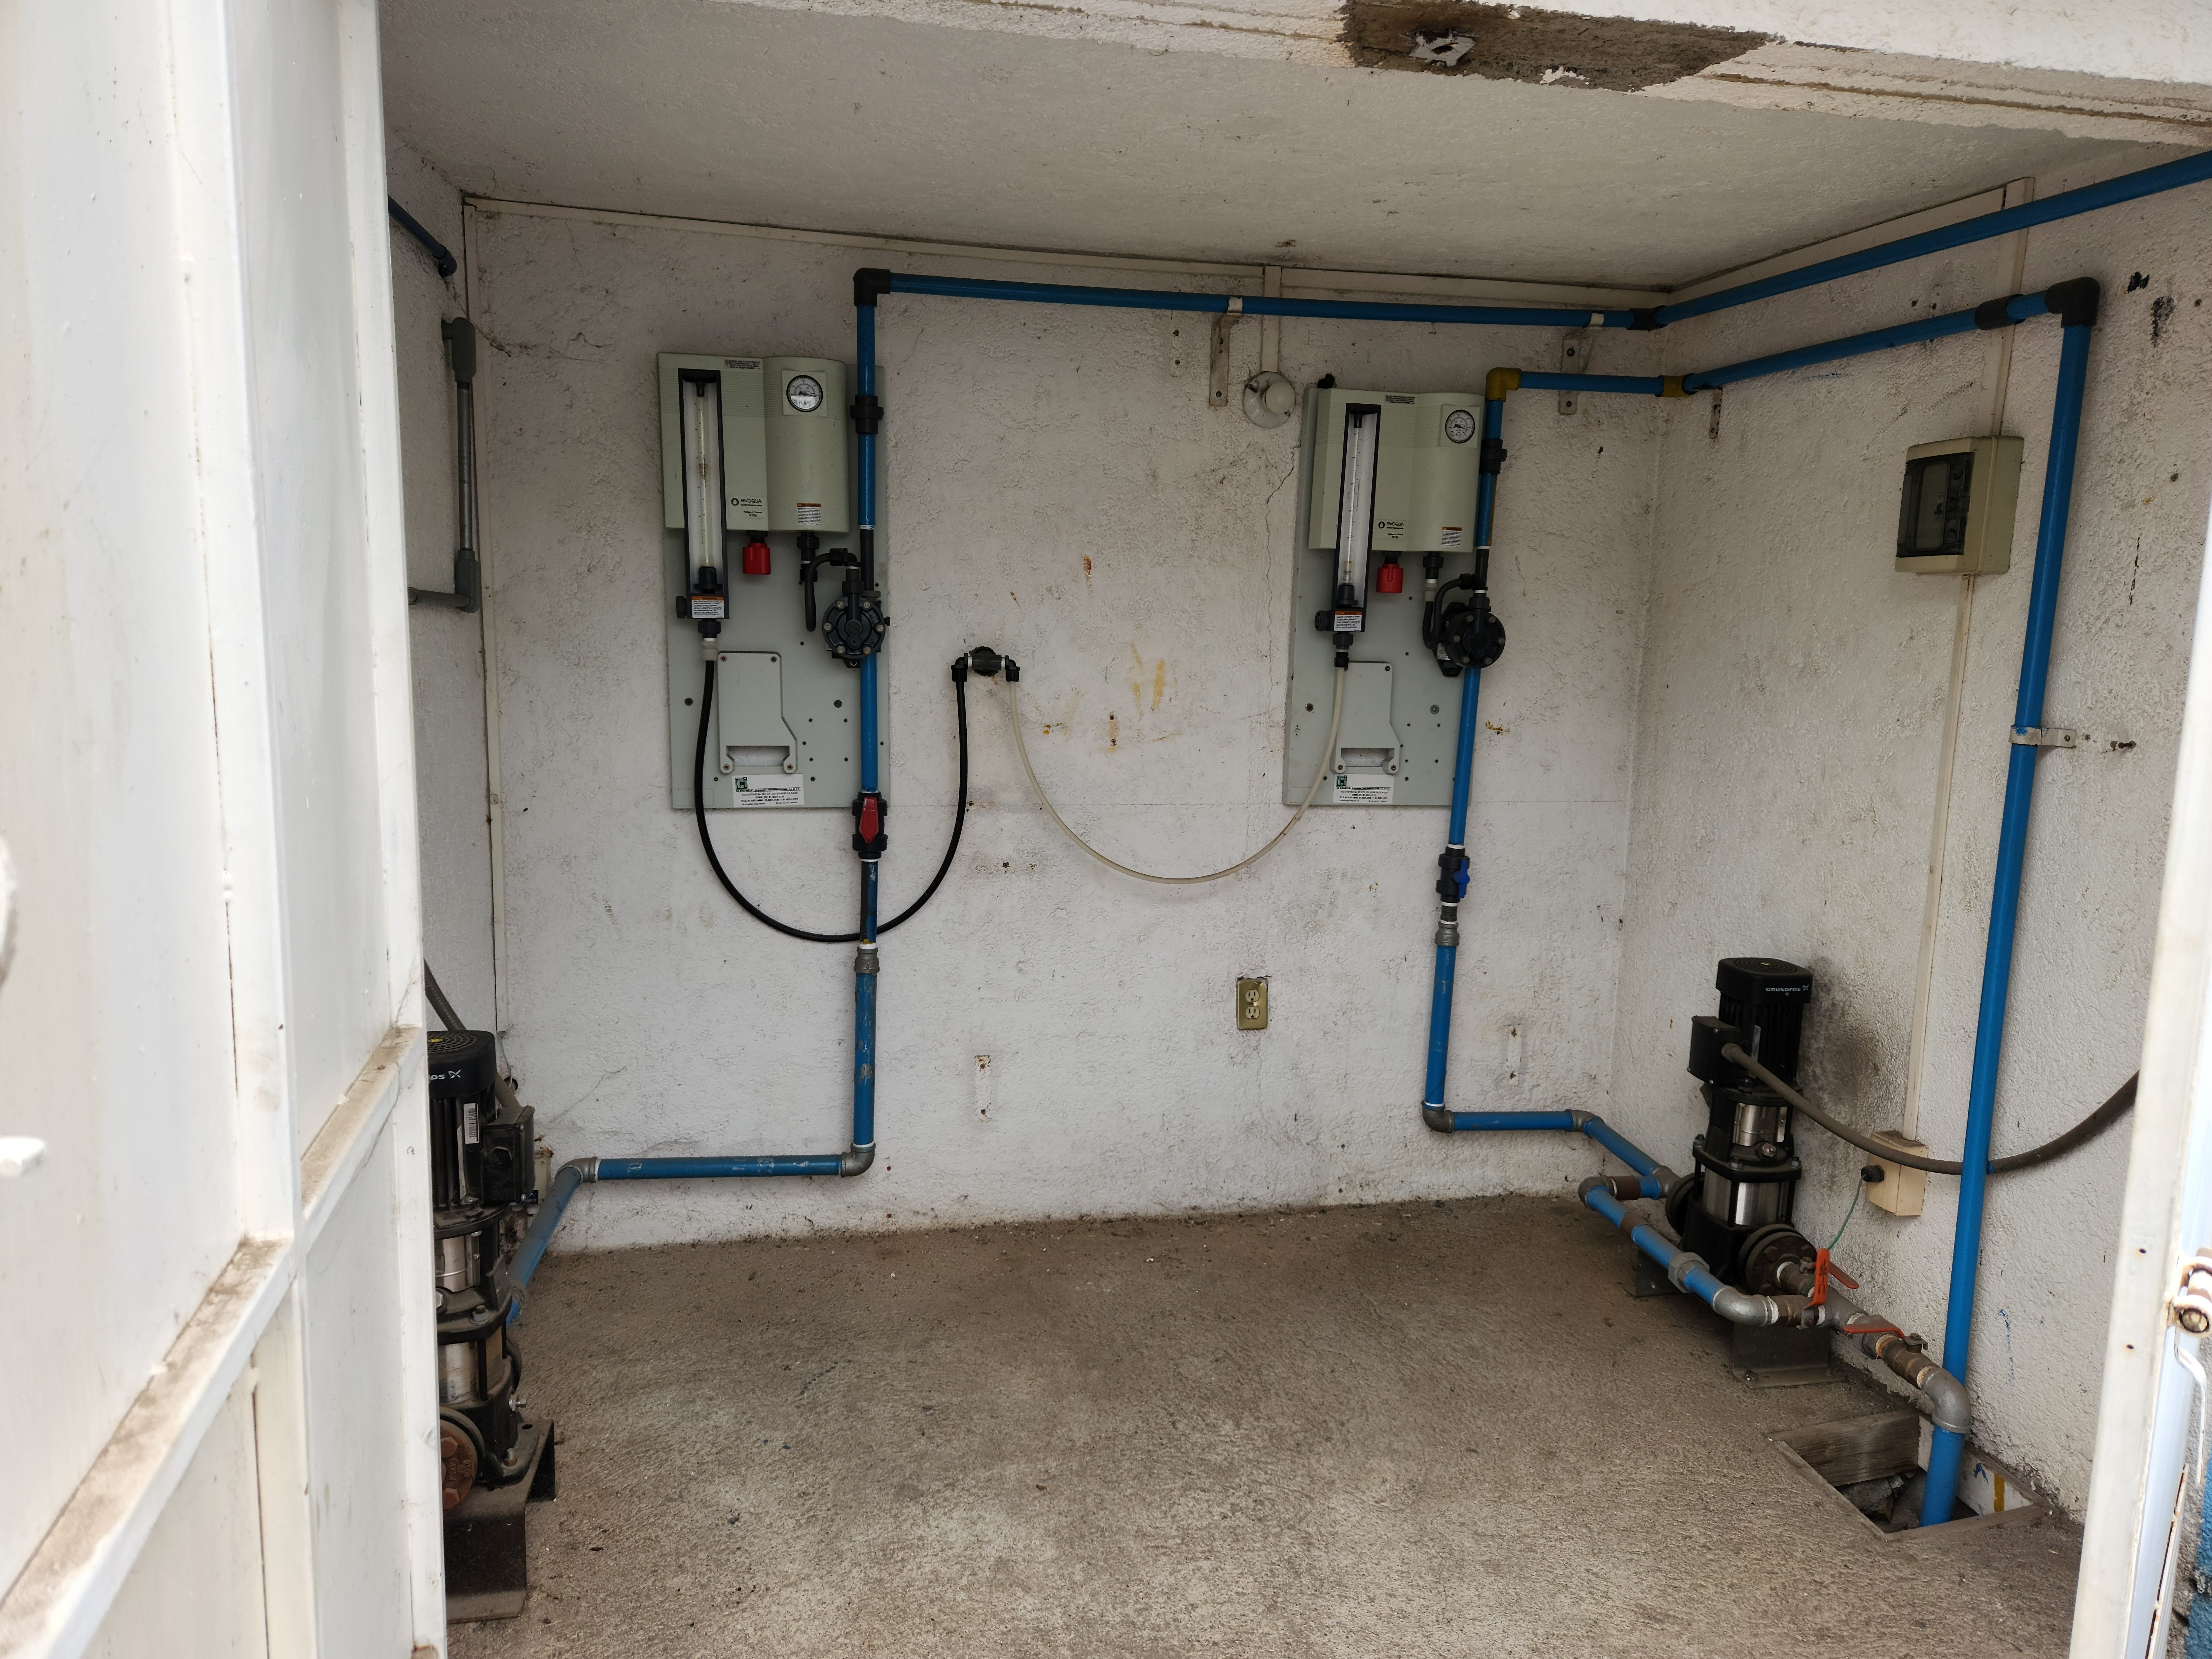
\includegraphics[scale=0.05,angle=0]{imgss15.jpg}
	\caption{Caseta de cloración}
	\label{fig:figura900_4}
\end{figure}

La adición de los reactivos desinfectantes es necesaria que se lleve a cabo en las etapas iniciales del proceso, de forma que se proporcione tiempo suficiente para que 
dichos reactivos logren eliminar la presencia bacteriológica antes de que el agua complete las etapas restantes de la potabilización y esté disponible para su distribución.

En esta etapa del proceso se ha comentado por parte del especialista del laboratorio de muestreo del OOAPAS que el nivel de calidad del agua presente en el agua cruda a la entrada de la planta es un factor determinante para 
poder tomar decisiones acerca de cómo debe realizarse la adición de agentes antibacteriológicos, particularmente en torno a la cantidad de sustancia a añadir. Por ejemplo, en época de lluvias cuando el agua cruda presenta un 
nivel de contaminación mayor, el proceso de desinfección debe mejorar para compensar esa mayor cantidad de material bacteriológico presente, lo cual se puede generar al elevar la cantidad de desinfectantes que se adicionan. Sin 
embargo, relacionado a esto también existe una restricción acerca de la cantidad de cloro que puede quedar presente en el agua potable una vez que ya se tiene el producto final del proceso. En esta parte nos tenemos que 
apoyar de la norma sanitaria correspondiente emitida por la Secretaria de Salud en conjunto con la Comisión Federal para la Protección contra Riesgos Sanitarios del Gobierno de México; la norma relativa para este caso específico 
es la Norma Oficial Mexicana NOM-127-SSA1. En ella se especifica que a la salida de un proceso de potabilización como el que se estudia en este proyecto el agua potable tiene un límite permisible para el cloro residual libre 
de 0.2mg/L a 1.5mg/L.
\clearpage
En la \autoref{fig:figura900_5} se muestran las siguientes etapas del proceso, los tanques de mezclado.

\begin{figure}[h]
	\centering
	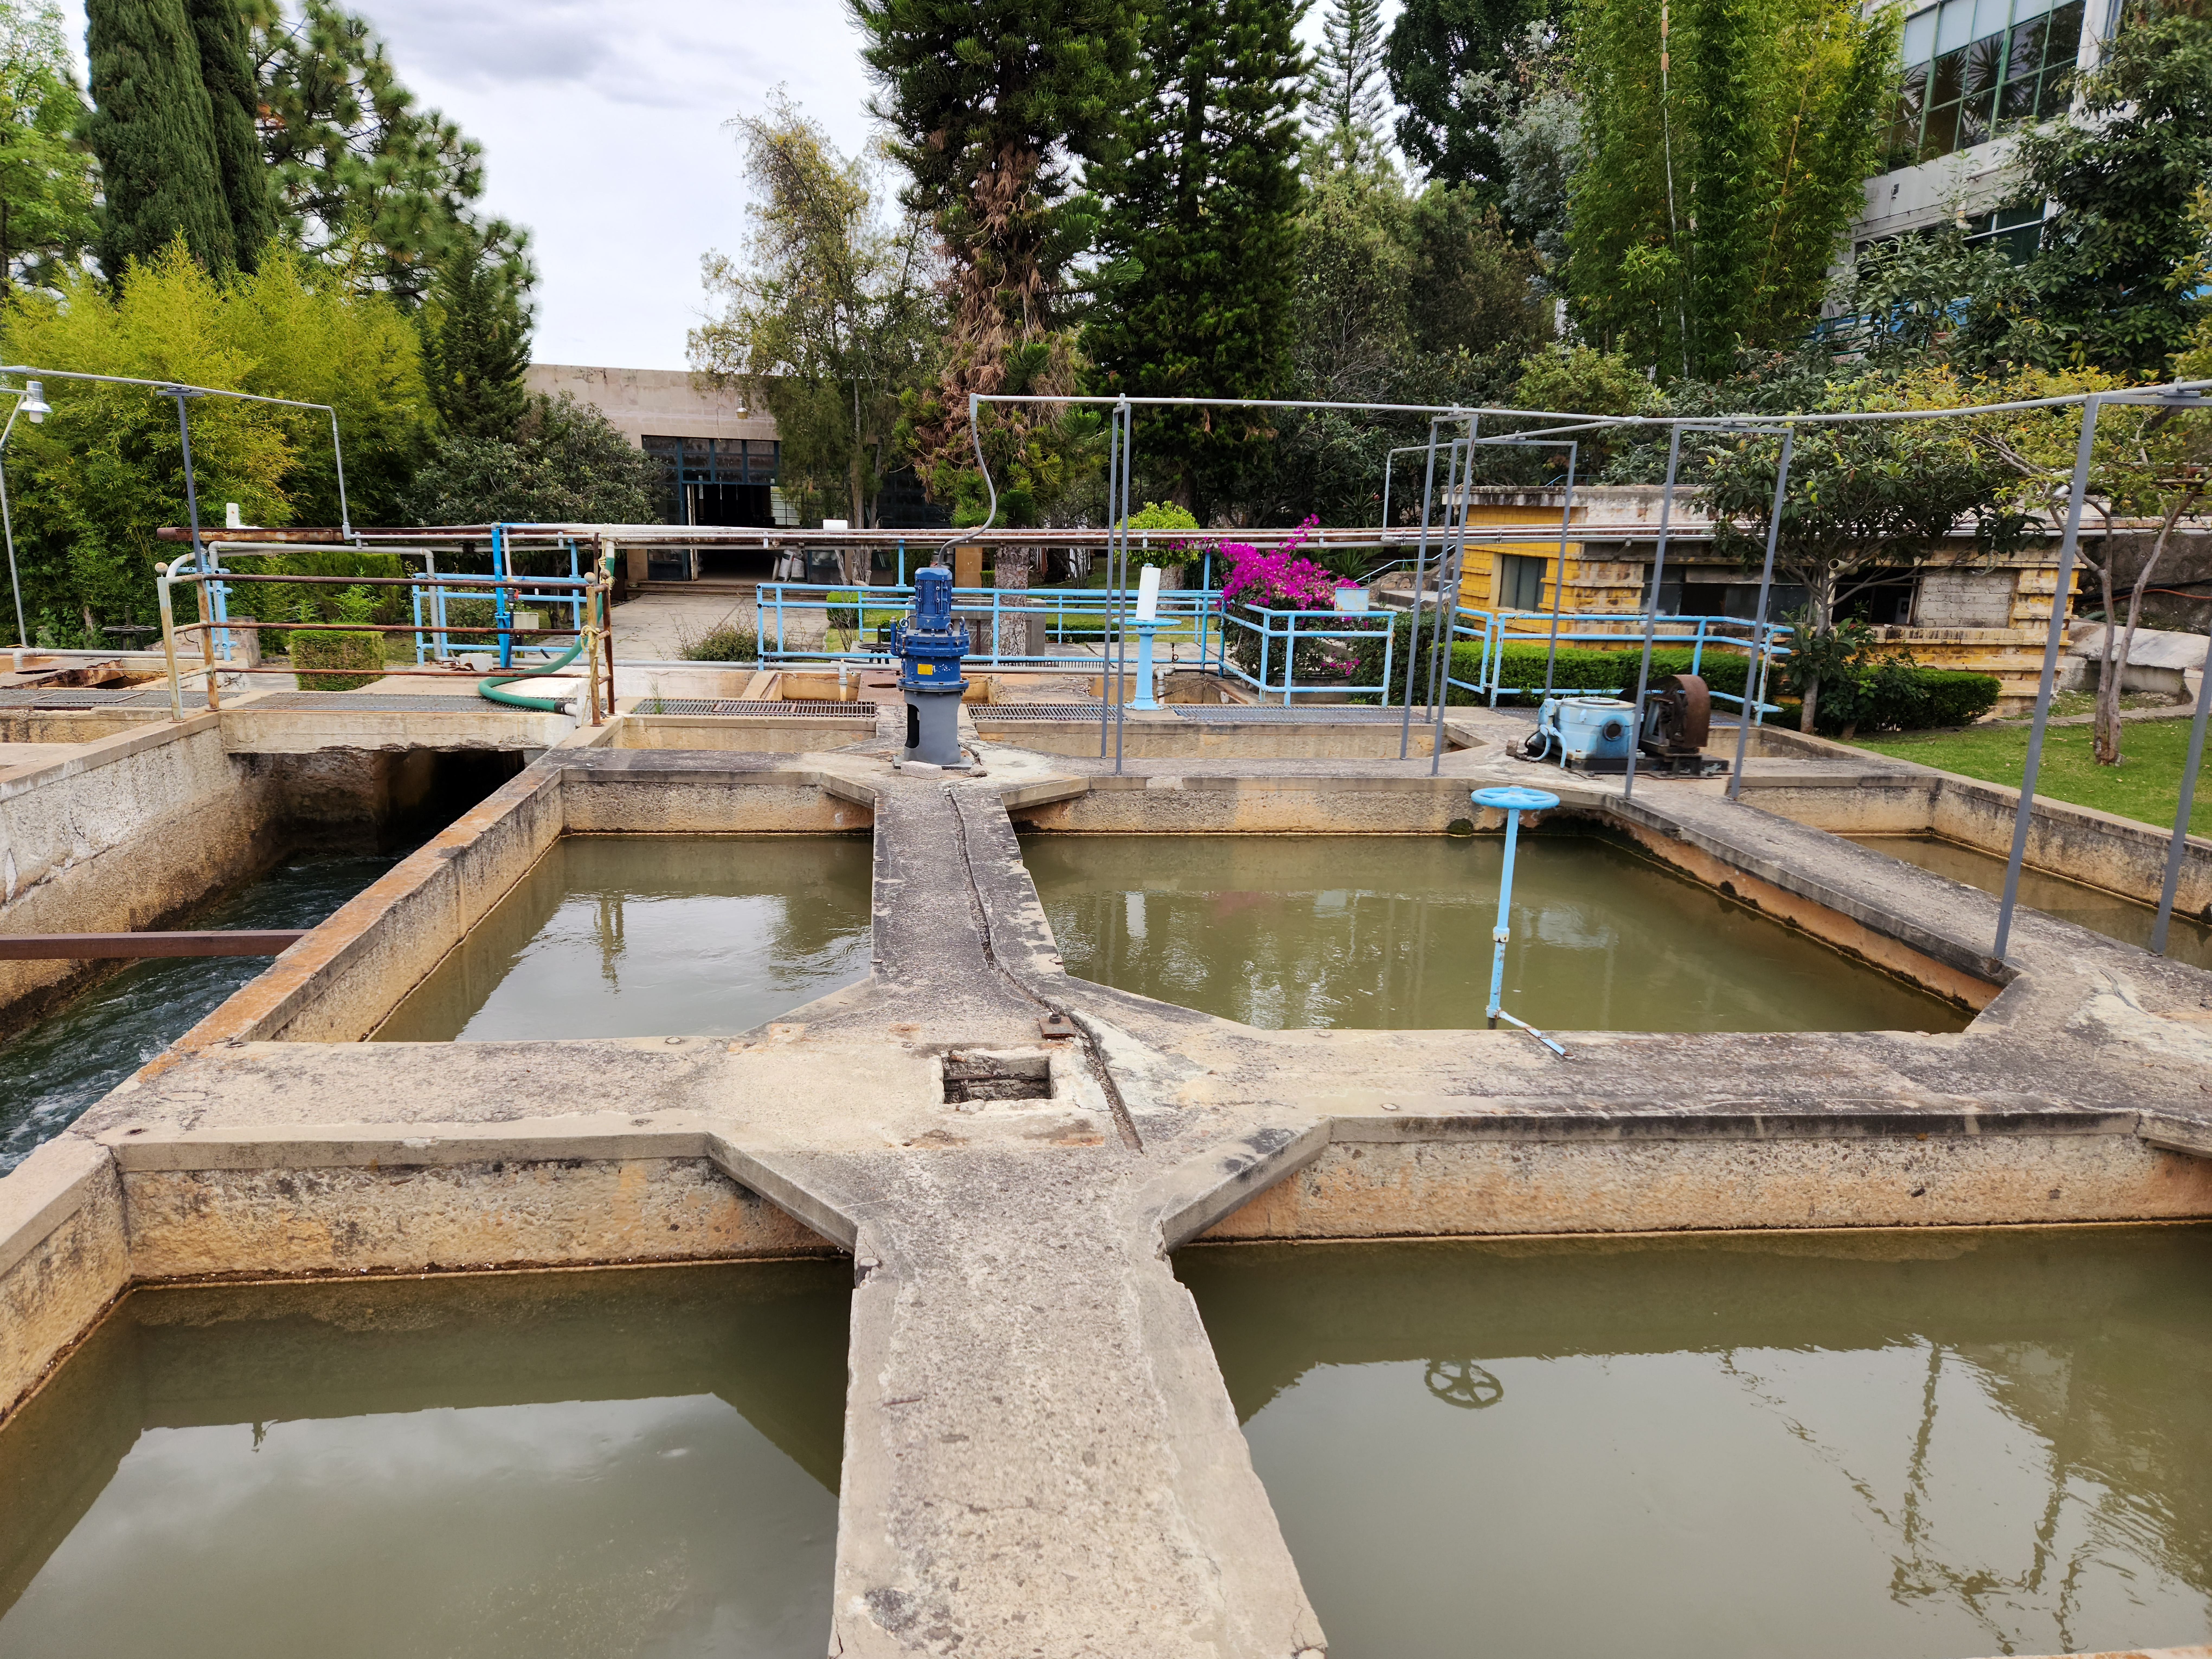
\includegraphics[scale=0.05,angle=0]{imgss16.jpg}
	\caption{Tanques de mezclado}
	\label{fig:figura900_5}
\end{figure}

Aquí se tienen 2 tipos: tanque de mezclado rápido y tanque de mezclado lento.

El tanque de mezclado rápido se utiliza con el fin de disolver adecuadamente los contaminantes que se encuentren presentes en el agua, mientras que el tanque de mezclado lento ayuda en el proceso de formación de flóculos 
con los contaminantes sólidos para su posterior eliminación.

En esta parte del proceso, los tanques de mezclado rápido han sido una de las 5 etapas de donde se han tomado muestras para obtener datos de los parámetros fisicoquímicos analizados. En este caso se ha elegido particularmente 
ese tanque para poder tener una caracterización próxima entre las condiciones en el agua cruda y las condiciones en este tanque de mezclado, es decir, analizar etapas consecutivas para tener información de los efectos inmediatos 
en la calidad del agua justo después de la adición del coagulante, floculante y los agentes de desinfección.


En la \autoref{fig:figura900_6} se muestra el canal de sedimentación, la etapa del proceso siguiente a los 2 tipos de tanque de mezclado.
\clearpage
\begin{figure}[h]
	\centering
	\includegraphics[scale=0.3,angle=0]{imgss17.jpg}
	\caption{Canal de sedimentación}
	\label{fig:figura900_6}
\end{figure}

Aquí se busca que toda la basura y contaminantes sólidos, una vez que ha terminado el proceso de floculación, puedan sedimentarse, es decir, que todo ese material sólido transportado por la corriente de agua, se pueda hundir 
o depositar en el fondo por efectos de gravedad. En esta etapa de separación de contaminantes se logra eliminar un porcentaje muy importante de los residuos presentes en el agua, ya que si se hace la compartiva de una muestra
correspondiente al canal de sedimentación contra una muestra de los tanques de mezclado, prácticamente todos los residuos de gran tamaño han desaparecido en la muestra correspondiente al canal, cuando la muestra de cualquiera
de los tanques de mezclado tiene presente una gran cantidad de flóculos formados por los contaminantes. Además el color del agua en cualquiera de los tanques es tonalidades cafés, y en el agua que se puede recolectar del 
canal de sedimentación ya existe una condición incolora.

\clearpage

Posteriormente, la etapa siguiente son los filtros, los cuales se muestran en la \autoref{fig:figura900_7}.

\begin{figure}[h]
	\centering
	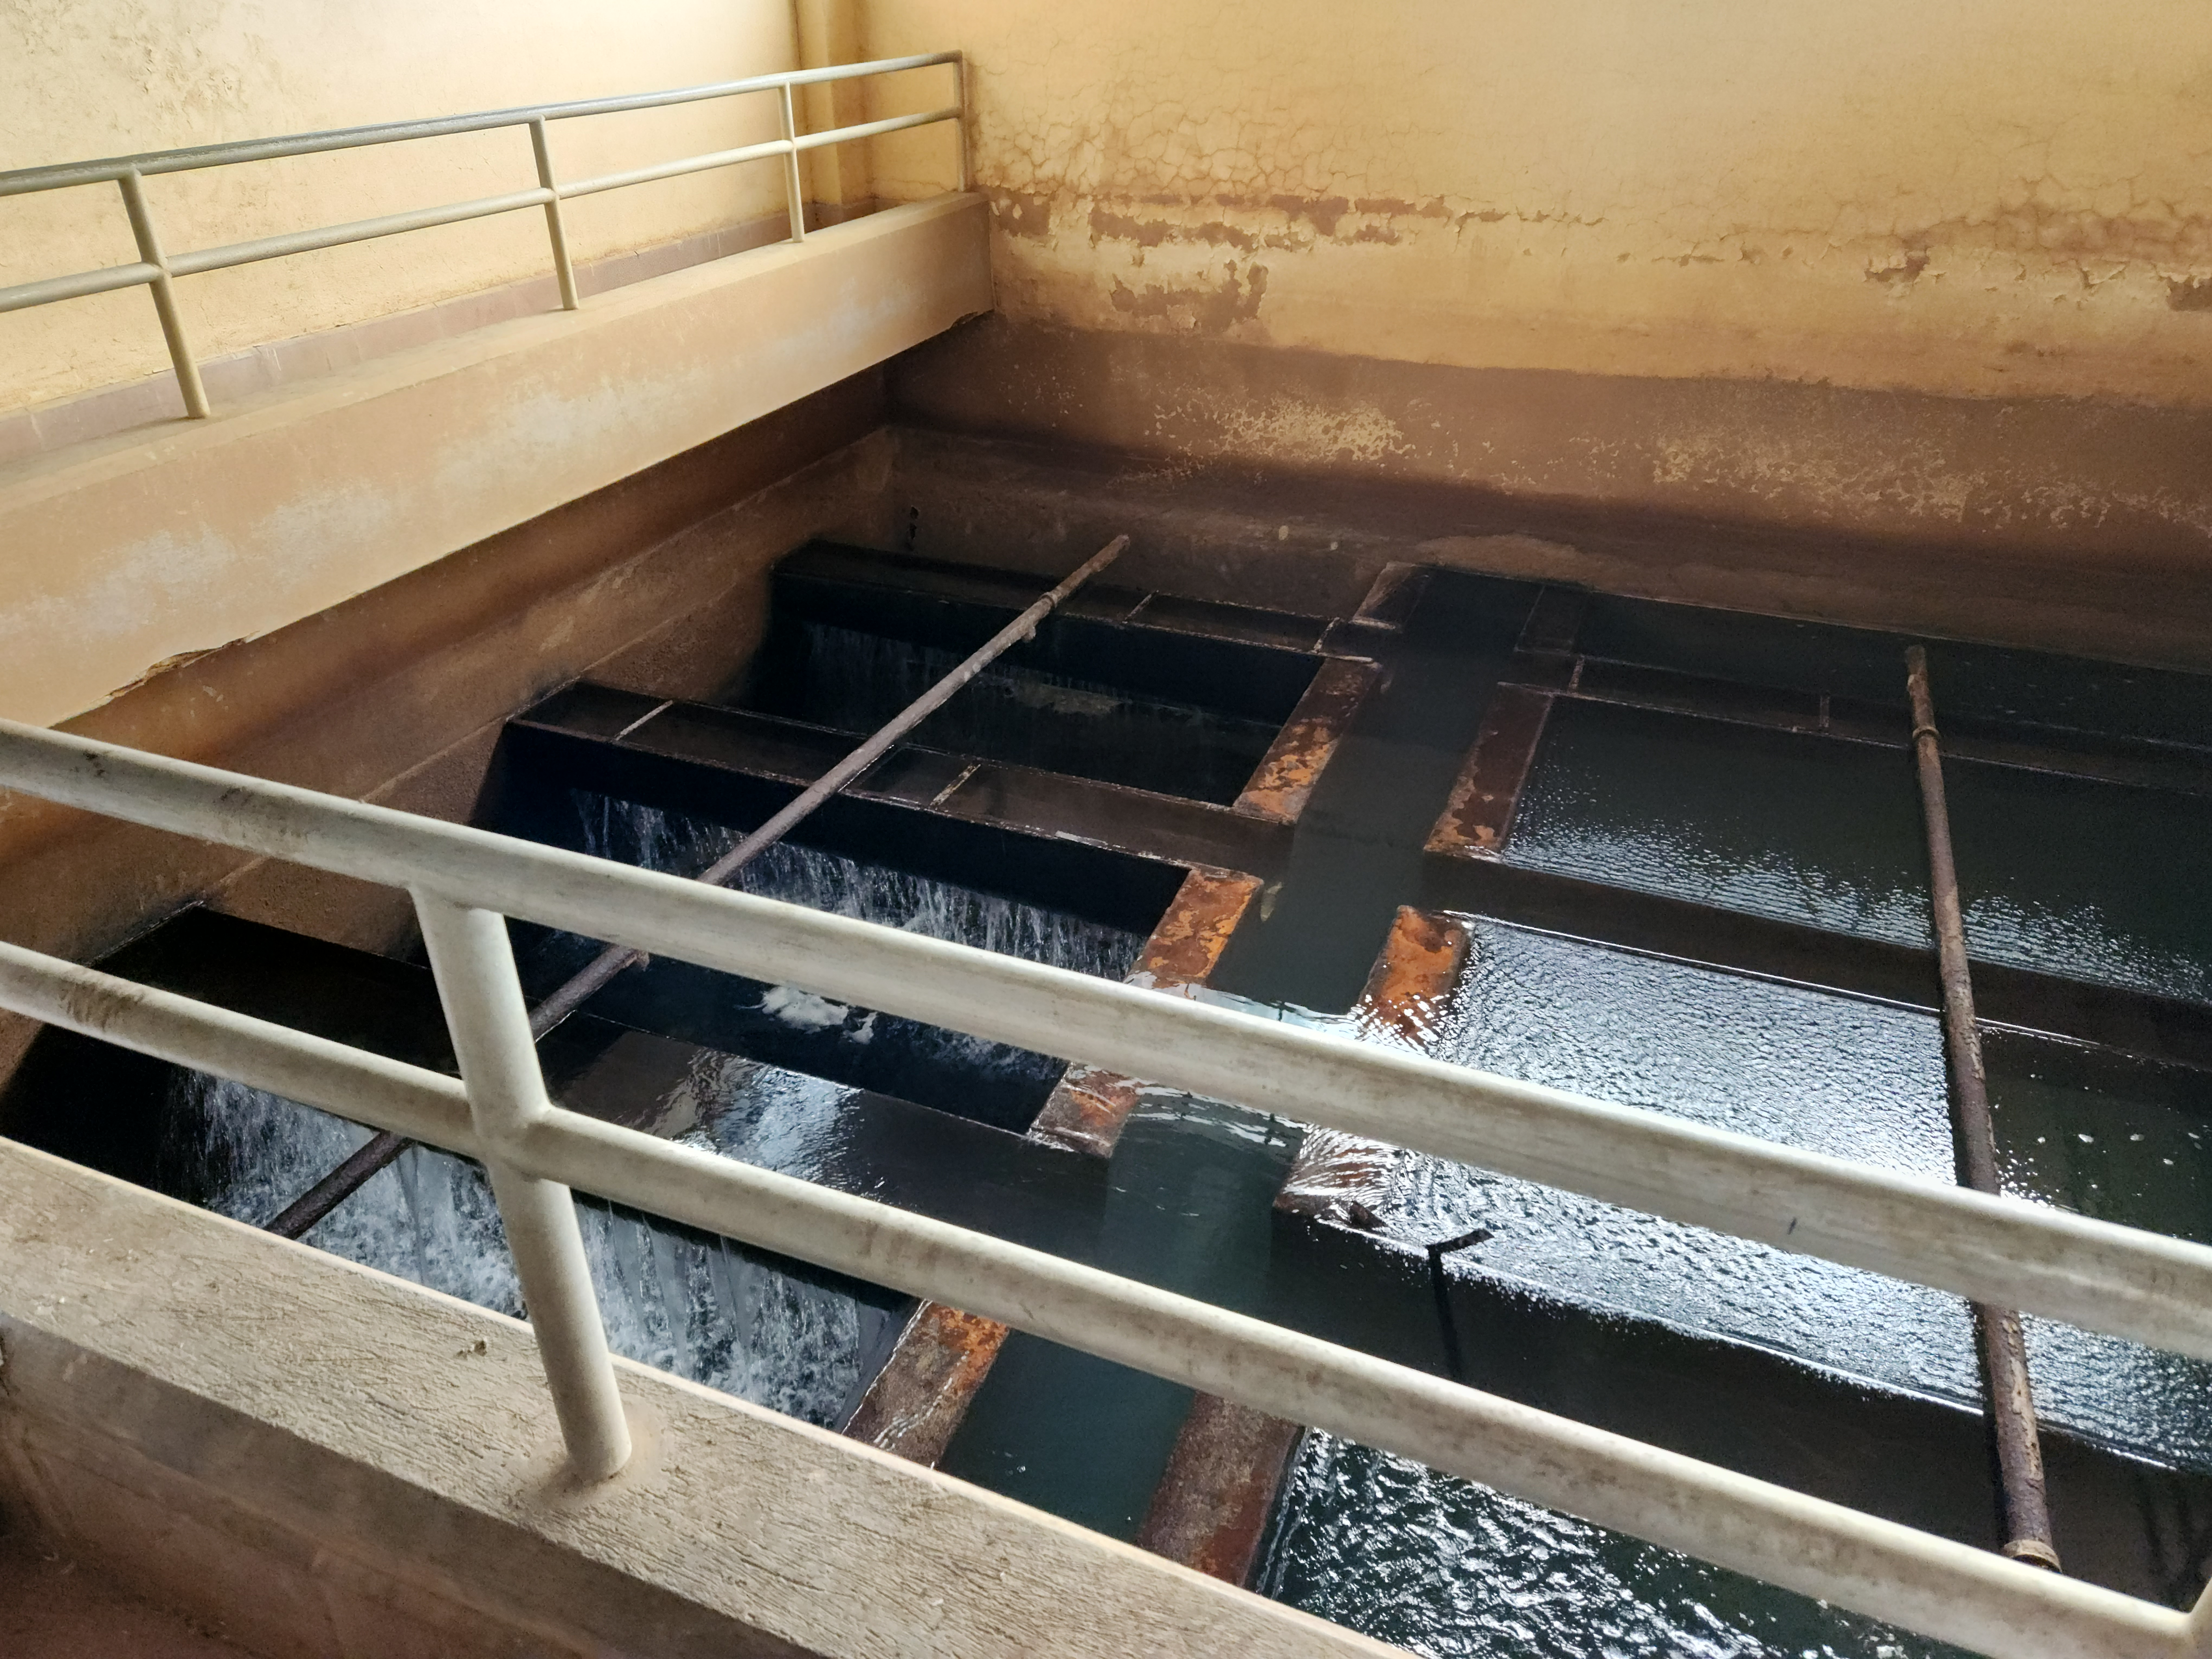
\includegraphics[scale=0.05,angle=0]{imgss18.jpg}
	\caption{Filtros}
	\label{fig:figura900_7}
\end{figure}

En la planta de potabilización se ha explicado que el tipo de filtrado realizado en este caso particular es el método de filtrado por gravedad, en el cual el líquido atraviesa un conjunto de capas, las cuales retienen las 
particulas sólidas que aún estén presentes. Estos filtros son la última etapa del proceso donde se ejecuta algún procedimiento físico para eliminación de contaminantes; la continuación del proceso después de esta última 
etapa de filtrado es un tanque de almacenamiento que se encuentra por debajo del suelo, en el cual el agua se almacena temporalmente una vez que ha terminado el filtrado.  

En la \autoref{fig:figura900_8} se muestran los canales que transportan el agua potabilizada lista para distribución.

\clearpage

\begin{figure}[h]
	\centering
	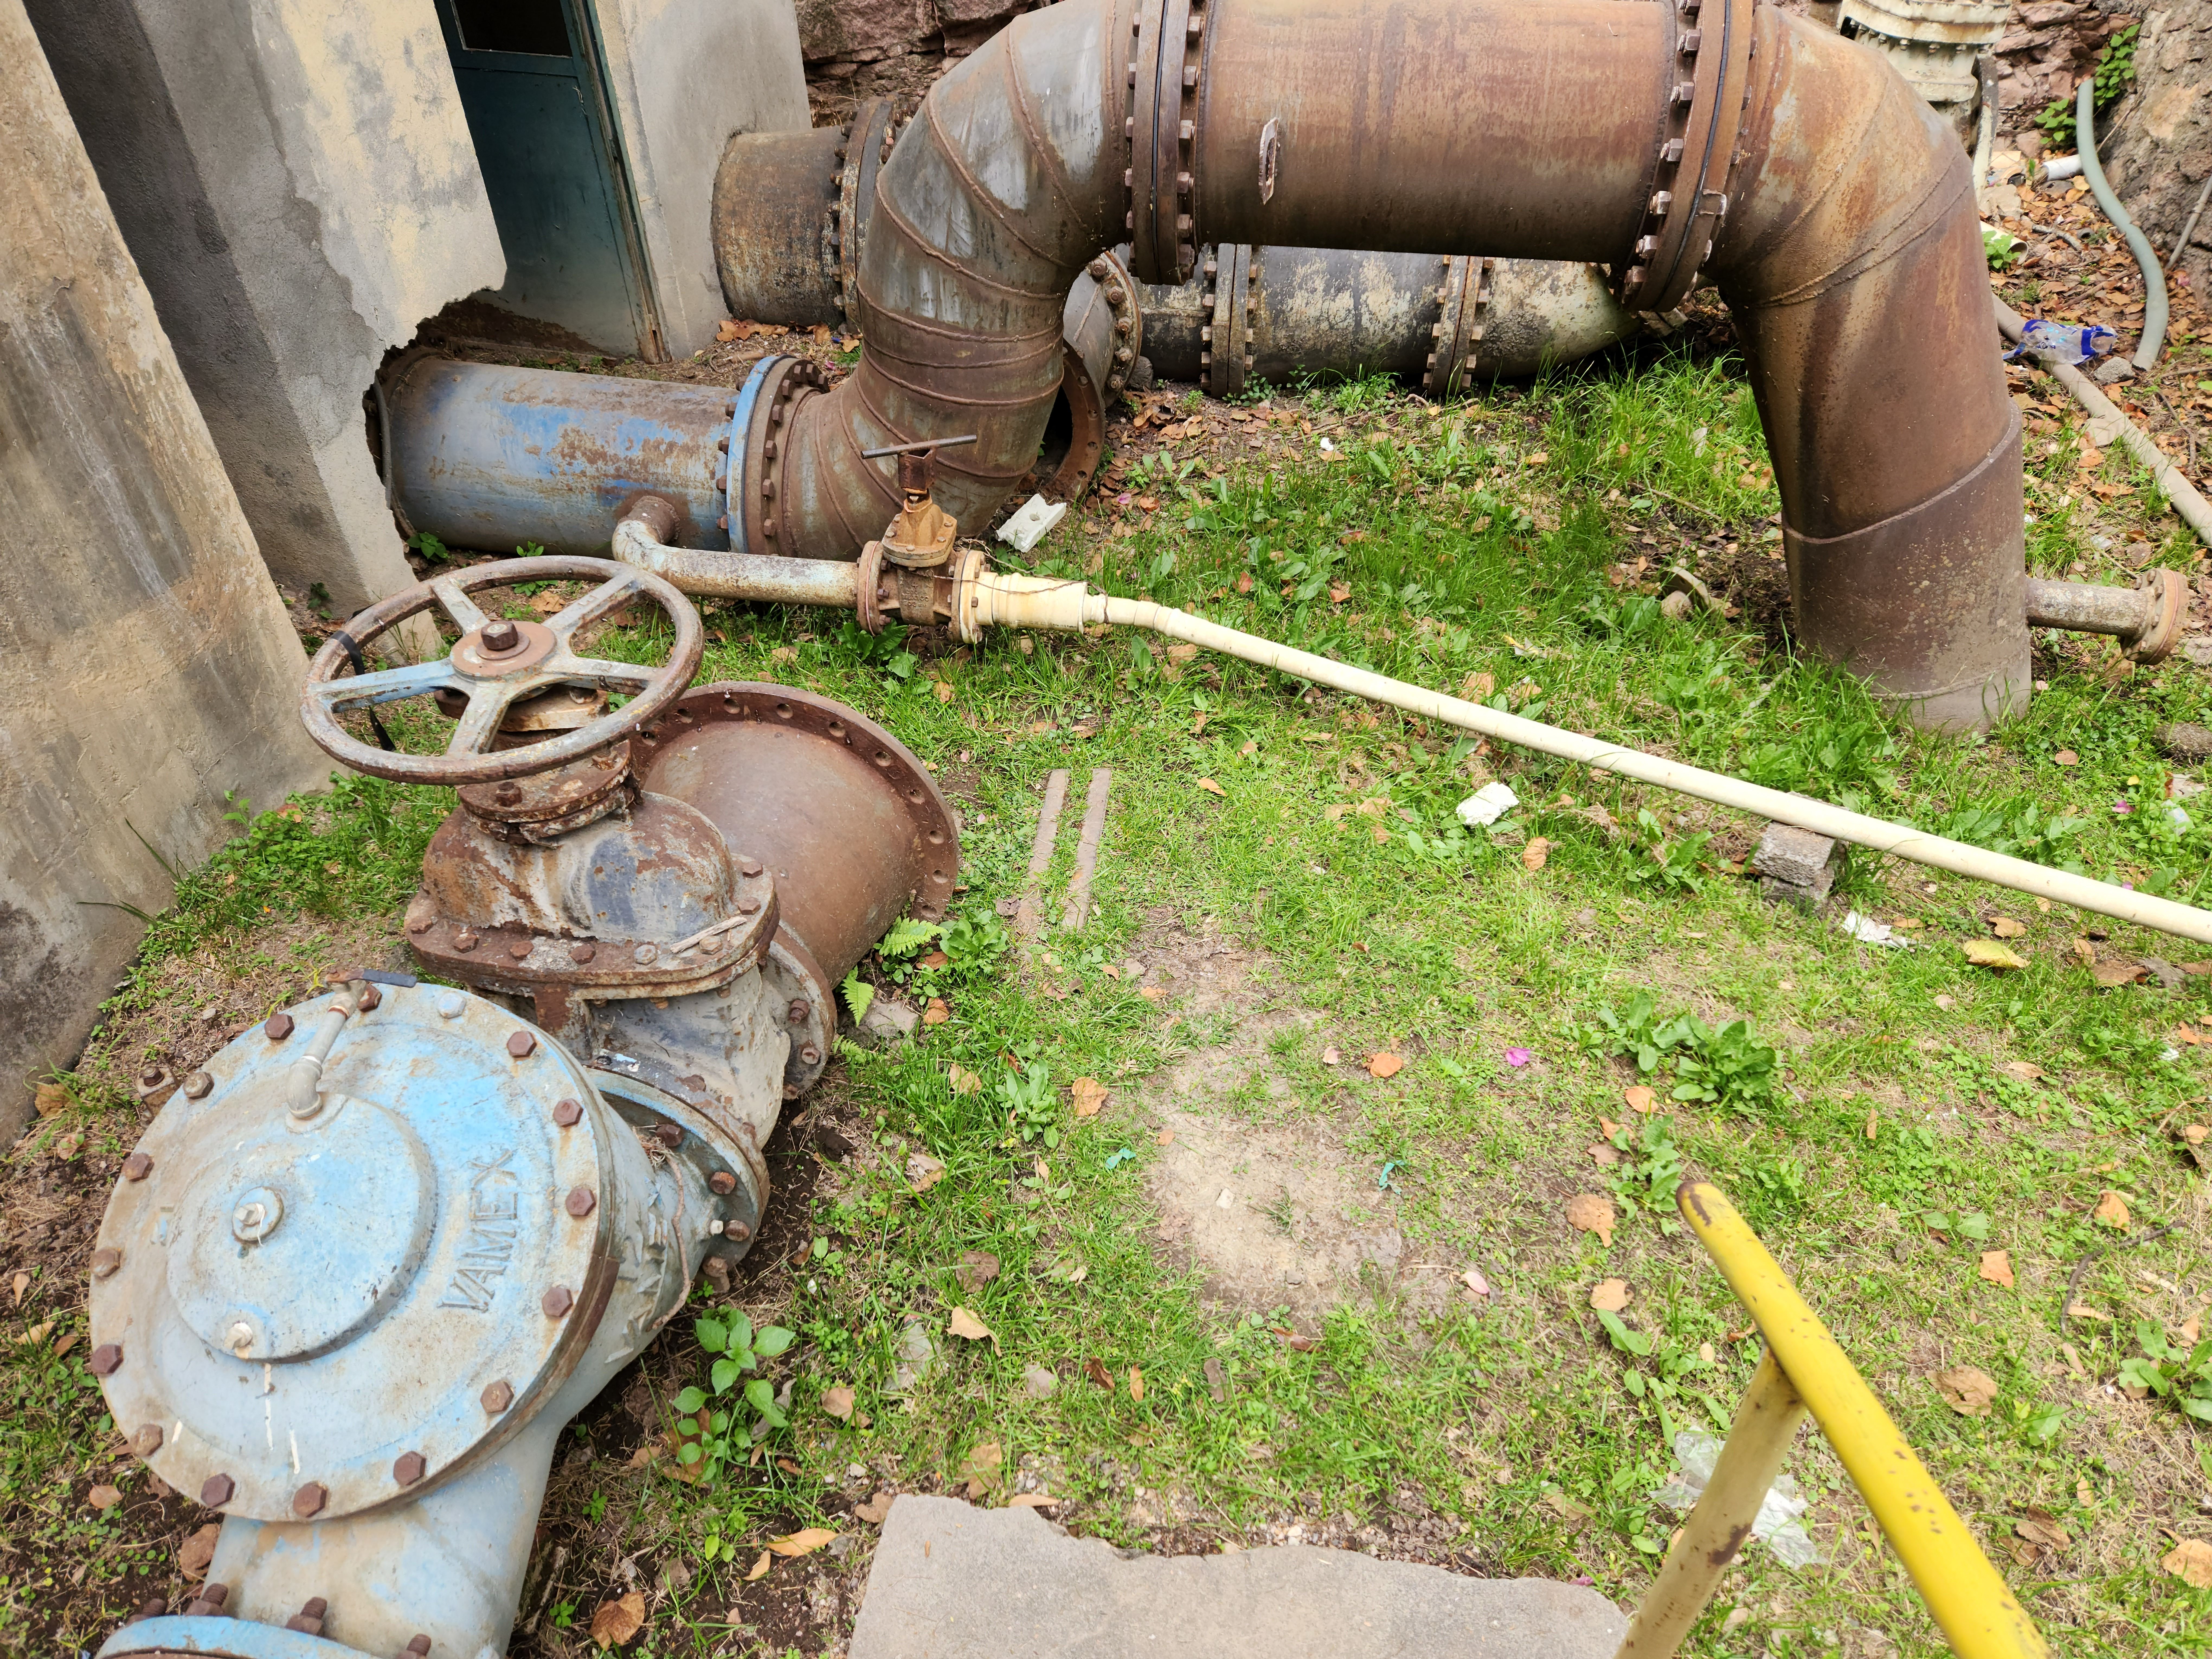
\includegraphics[scale=0.05,angle=0]{imgss19.jpg}
	\caption{Salida del proceso, agua potable}
	\label{fig:figura900_8}
\end{figure}

Es por estos canales por donde el agua pasa al sistema de distribución después de haber estado en el tanque de almacenamiento una vez que terminó el filtrado. 

Por lo tanto, de forma general el proceso consiste primeramente en la adición de los reactivos para coagulación y floculación, de forma que en los tanques de mezclado y el canal de 
sedimentación pueda quedar atrapada la mayor parte de los componentes sólidos. Además, inicalmente también se han agregado los desinfectantes para que estos actuen durante el proceso
y al final del mismo, el proceso de desinfección tuviese el tiempo suficiente para llevarse a cabo adecuadamente. Finalmente, antes de la salida del proceso donde ya se tiene agua potable para 
distribución, también se realiza la etapa de filtrado donde se retienen las partículas más pequeñas que no pudieron ser eliminadas por sedimentación.

Ahora, en lo referente al seguimiento preventivo que realiza el OOAPAS para vigilar el estado del conjunto de parámetros de calidad del agua que ellos manejan, se sigue un proceso diario de recolección de muestras en diferentes 
puntos del proceso. Esta toma de muestras es realizada por las mañanas y el líquido recolectado es llevado a los laboratorios de la planta para realizar pruebas de bacteriología, pruebas de propiedades químicas y propiedades 
físicas. Con estos ensayos es que se puede verificar el cumplimiento de la normativa que regula este tipo de proceso de tratamiento, que se tiene específicamente la regulación NOM-127-SSA1-2021 de agua para uso y consumo 
humano y sus límites permisibles de calidad.

\section{Conclusiones}

Este proyecto tiene como uno de sus propósitos el realizar mediciones para diversas variables de calidad del agua en el proceso de potabilización del OOAPAS. Es importante que previamente a comenzar la toma de muestras, 
se tenga el entendimiento acerca las partes que componen el proceso que se va a estudiar. En este capítulo se presenta la descripción etapa por etapa del proceso a caracterizar, haciendo uso de imágenes y explicando la función 
o propósito específico de cada fase del proceso, lo cual ayuda a relacionar las diferentes etapas al comprender los cambios que se van produciendo conforme fluye el líquido por el proceso, logrando identificar la dependencia 
que existe entre dichas etapas.
